\section{Grid-based Methods}

\begin{frame}{Grid-based Clustering Method}
	\begin{itemize}
		\item \textbf{Using multi-resolution grid data structure.}
		\item \textbf{Several interesting methods.}
		\begin{itemize}
			\item STING (a STatistical INformation Grid approach) (Wang, Yang 
			\& Muntz, VLDB'97).
			\item WaveCluster (Sheikholeslami, Chatterjee \& Zhang, VLDB'98):
			\begin{itemize}
				\item A multi-resolution clustering approach using wavelet 
				method.
				\item Not shown here.
			\end{itemize}
			\item CLIQUE (Agrawal et al., SIGMOD'98):
			\begin{itemize}
				\item Both grid-based and subspace clustering.
			\end{itemize}
		\end{itemize}
	\end{itemize}
\end{frame}

\begin{frame}{STING: A Statistical Information Grid Approach}
	\begin{itemize}
		\item \textbf{The spatial area is divided into rectangular cells.}
		\item \textbf{There are several levels of cells corresponding to 
		different levels of resolution.}
		\item (Wang, Yang \& Muntz, VLDB'97)
	\end{itemize}
	\vspace{0.5cm}
	\centering
	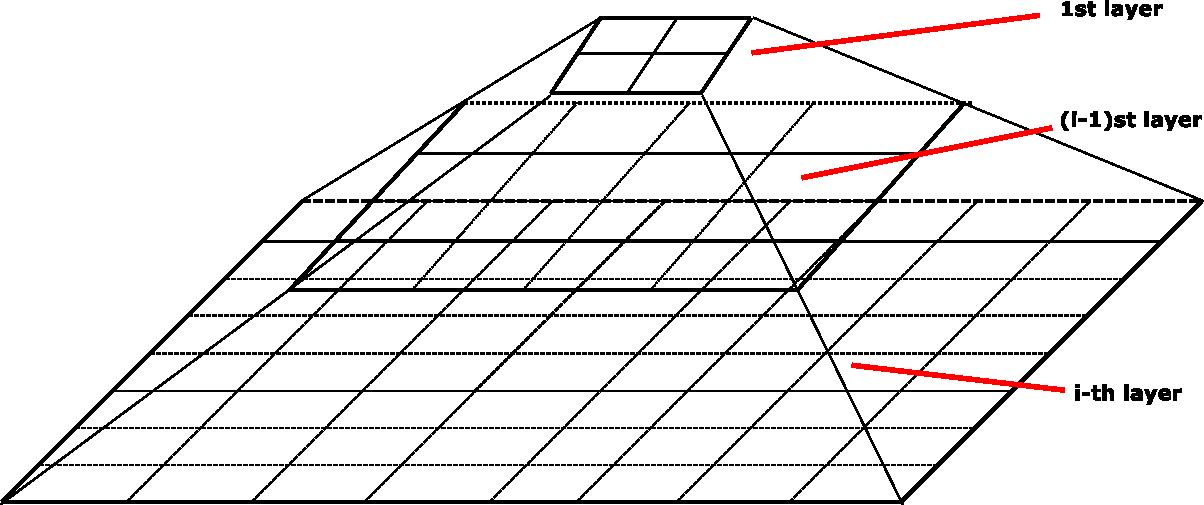
\includegraphics[width=10cm]{img/layers.pdf}
\end{frame}

\begin{frame}{The STING Clustering Method (I)}
	\begin{itemize}
		\item \textbf{Each cell at a higher level:}
		\begin{itemize}
			\item Partitioned into a number of smaller cells at next lower 
			level.
		\end{itemize}
		\item \textbf{Statistical info of each cell:}
		\begin{itemize}
			\item Calculated and stored beforehand and used to answer queries.
			\item Count, plus for each attribute: mean, standard dev, min, max 
			and \\
			type of distribution: normal, uniform, etc.
		\end{itemize}
		\item \textbf{Parameters of higher-level cells:}
		\begin{itemize}
			\item Can easily be calculated from parameters of lower-level cells.
		\end{itemize}
		\item \textbf{Use a top-down approach:}
		\begin{itemize}
			\item To answer spatial data queries (or: cluster definitions).
		\end{itemize}
		\item \textbf{Start from a pre-selected layer:}
		\begin{itemize}
			\item Typically with a small number of cells.
		\end{itemize}
		\item \textbf{For each cell at the current level:}
		\begin{itemize}
			\item Compute the confidence interval.
		\end{itemize}
	\end{itemize}
\end{frame}

\begin{frame}{The STING Clustering Method (II)}
	\begin{itemize}
		\item \textbf{Cells labeled relevant or not relevant.}
		\begin{itemize}
			\item At the specified confidence level.
			\item Irrelevant cells removed from further consideration.
		\end{itemize}
		\item \textbf{When finished examining the current layer, proceed to the 
		next lower level.}
		\begin{itemize}
			\item Only look at cells that are children of relevant cells.
		\end{itemize}
		\item \textbf{Repeat this process until bottom layer is reached.}
		\item \textbf{Find regions (clusters) that satisfy the 
		{\color{airforceblue}density} specified.}
		\begin{itemize}
			\item Breadth-first search, at bottom layer.
			\item Examine cells within a certain distance from center of 
			current cell (often just the neighbors).
			\item If average density within this small area is greater than 
			density specified, mark area and put relevant cells just examined 
			into queue.
			\item Examine next cell from queue and repeat procedure, until end 
			of queue.
			\item Then one region has been identified.
		\end{itemize}
	\end{itemize}
\end{frame}

\begin{frame}{STING Algorithm: Analysis}
	\begin{itemize}
		\item \textbf{Advantages:}
		\begin{itemize}
			\item Query-independent, easy to parallelize, incremental update.
			\item $\mathcal{O}(K)$, where $K$ is the number of grid cells at 
			the lowest level.
		\end{itemize}
		\item \textbf{Disadvantages:}
		\begin{itemize}
			\item All the cluster boundaries are either horizontal or vertical, 
			\\
			and no diagonal boundary is detected.
		\end{itemize}
	\end{itemize}
\end{frame}

\begin{frame}{CLIQUE (CLustering In QUEst)}
	\begin{itemize}
		\item \textbf{Using {\color{airforceblue}subspaces} (lower-dimensional) 
		of a high-dimensional data space that allow better clustering than 
		original space:}
		\begin{itemize}
			\item (Agrawal, Gehrke, Gunopulos \& Raghavan, SIGMOD'98).
		\end{itemize}
		\item \textbf{CLIQUE can be considered as both density-based and 
		grid-based.}
		\begin{itemize}
			\item Partitions each dimension into non-overlapping intervals, \\
			thereby partitioning the entire data space into \textbf{cells}.
			\item Uses density threshold to identify \textbf{dense} cells.
			\begin{itemize}
				\item A cell is dense, if the number of data points mapped to 
				it exceeds the density threshold.
			\end{itemize}
		\end{itemize}
	\end{itemize}
\end{frame}

\begin{frame}{CLIQUE: The Major Steps (I)}
	\begin{itemize}
		\item \textbf{Monotonicity of dense cells w.r.t. dimensionality:}
		\begin{itemize}
			\item Based on the a priori property used in frequent-pattern and 
			association-rule mining (see Chapter 5).
			\item $k$-dimensional cell $c$ can have at least $l$ points only, 
			if every $(k-1)$-dimensional projection of $c$ (which is a cell in 
			a $(k-1)$-dimensional subspace) has at least $l$ points, too.
		\end{itemize}
		\item \textbf{Clustering step 1:}
		\begin{itemize}
			\item Partition each dimension into intervals, identify intervals 
			containing at least $l$ points.
			\item Iteratively join $k$-dimensional dense cells $c_1$ and $c_2$ 
			in subspaces $(D_{i1}, \ldots, D_{ik})$ and $(D_{j1}, \ldots, 
			D_{jk})$ with $D_{i1} = D_{j1}$ and $D_{i2} = D_{j2}$ and $\ldots 
			D_{i(k-1)} = D_{j(k-1)}$ and $c_1$ and $c_2$ share the same 
			intervals to those dimensions.
			\item New $(k+1)$-dimensional candidate cell $c$ in space $(D_{i1}, 
			\ldots, D_{ik}, D_{jk})$ tested for density.
		\end{itemize}
	\end{itemize}
\end{frame}

\begin{frame}{CLIQUE: The Major Steps (II)}
	\begin{itemize}
		\item \textbf{Clustering step 1 (cont.):}
		\begin{itemize}
			\item Iteration terminates when no more candidate cells can be 
			generated or no candidate cells are dense.
		\end{itemize}
		\item \textbf{Clustering step 2:}
		\begin{itemize}
			\item Use dense cells in each subspace to assemble clusters.
			\item Apply Minimum Description Length (MDL) principle to use the 
			maximal regions to cover connected dense cells.
			\begin{itemize}
				\item \textbf{\color{airforceblue}Maximal region}: hyper 
				rectangle where every cell falling into the regions is dense, 
				and region cannot be extended further in any dimension.
			\end{itemize}
			\item Simple greedy approach:
			\begin{itemize}
				\item Start with arbitrary dense cell.
				\item Find maximum region covering that cell.
				\item Work on remaining dense cells that have not yet been 
				covered.
			\end{itemize}
		\end{itemize}
	\end{itemize}
\end{frame}

\begin{frame}{CLIQUE: Example}
	\centering
	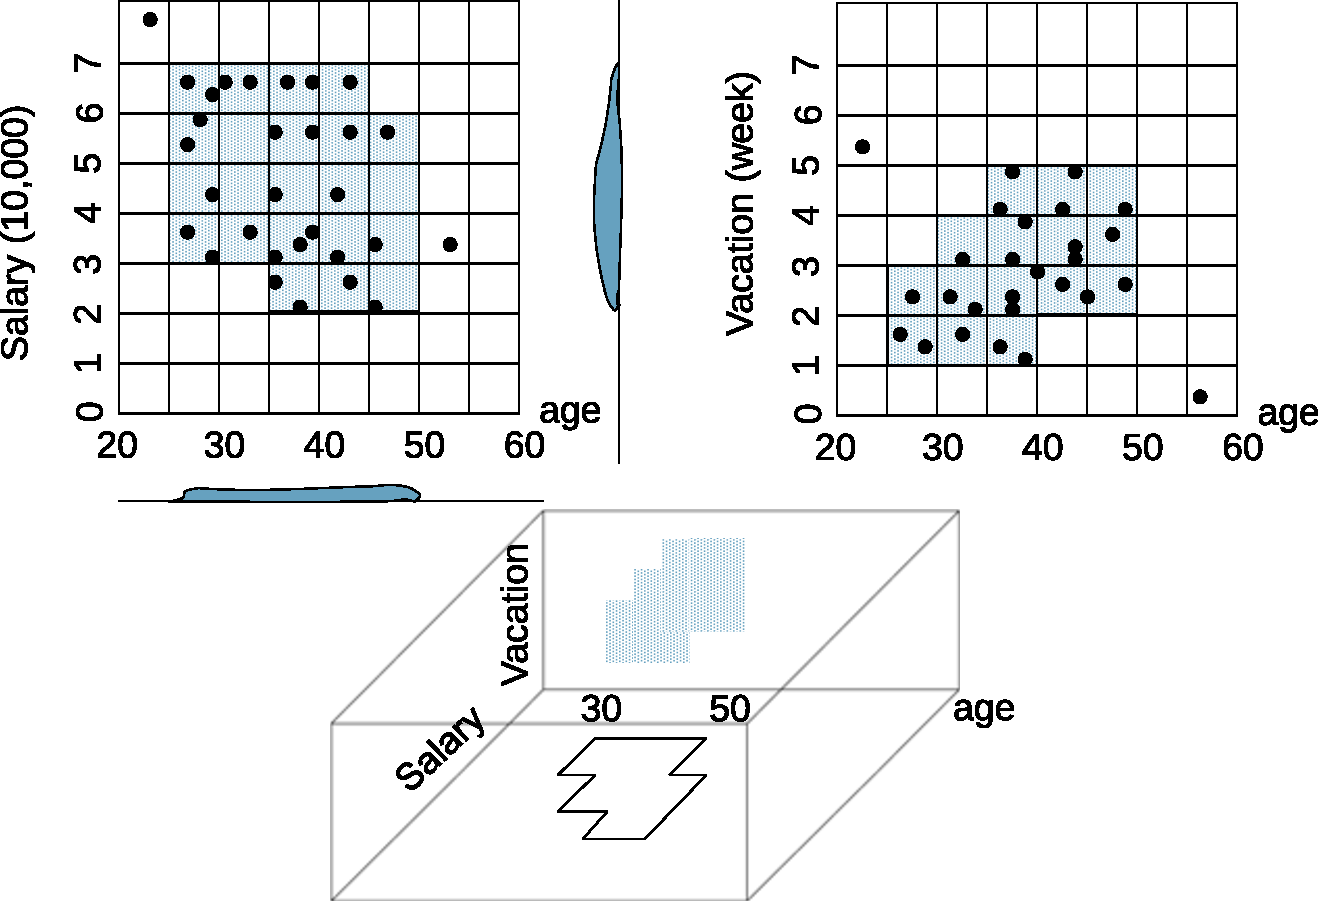
\includegraphics[width=9cm]{img/clique.pdf}
\end{frame}

\begin{frame}{Strength and Weakness of CLIQUE}
	\begin{itemize}
		\item \textbf{Strength:}
		\begin{itemize}
			\item Automatically finds subspaces of the highest dimensionality \\
			such that high-density clusters exist in those subspaces.
			\item Insensitive to the order of records in input and does not 
			presume \\
			any canonical data distribution.
			\item Scales linearly with the size of input and has good 
			scalability \\
			as the number of dimensions in the data is increased.
		\end{itemize}
		\item \textbf{Weaknesses:}
		\begin{itemize}
			\item Dependent on proper grid size and density threshold.
			\item Accuracy of clustering result may be degraded at the expense 
			\\
			of simplicity of the method.
		\end{itemize}
	\end{itemize}
\end{frame}